\documentclass[a4paper,12pt]{article}


%-----数学宏包-----
\usepackage{amsmath,amsthm,amssymb,amsfonts}
\usepackage{mathrsfs,bm}
%-----draft下 label提示-----
%\usepackage[notcite,notref]{showkeys}
%-----页面布局-----
\usepackage{geometry}
% \geometry{left=1.25in,right=1.25in,top=1in,bottom=1in}
%\geometry{left=1in,right=1in,top=1in,bottom=1in}
%\geometry{left=2.5cm,right=2.1cm,top=1.7cm,bottom=2cm,includehead,includefoot}
\geometry{
  left=2.54cm,        % 左边距
  right=2.54cm,       % 右边距
  top=2.54cm,         % 上边距
  bottom=2.54cm       % 下边距
}
%-----设置超链接-----
\usepackage{url,hyperref}
\hypersetup{colorlinks=true,linkcolor=black,citecolor=black} % 去掉目录红框
%-----制作目录-----
\usepackage{imakeidx}
% 设置颜色
\usepackage{color,xcolor}
% 插入图片
\usepackage{graphicx}
\usepackage{epsfig}
%-----设置表格-----
\usepackage{tabularx,array}
\usepackage{longtable}
\usepackage{booktabs}
\usepackage{multirow}
\usepackage{multicol}
\usepackage{fancybox}
%-----调整单元格格式-----
\usepackage{makecell}
%-----操作字符串-----
\usepackage{xstring}
%-----多语种处理-----
%\usepackage[english]{babel}
%-----设置代码环境-----
\usepackage{listings}
%-----设置章节标题和目录-----
\usepackage{titletoc}
\usepackage{titlesec}
%-----数学公式扩展-----
\usepackage{mathtools}
%-----浮动体设置-----
\usepackage{float}
%-----书签设置-----
\usepackage{bookmark}
%-----参考文献格式-----
\usepackage[numbers]{natbib}
%-----设置页眉页脚格式-----
\usepackage{fancyhdr}
\setlength{\parindent}{0pt}
%-----设置行间距 -----
\renewcommand*{\baselinestretch}{1.5}

%\setmainfont{Times New Roman}
%\setmonofont{Courier New}
%\setsansfont{Arial}
%\setCJKfamilyfont{kai}[AutoFakeBold]{simkai.ttf}
%\newcommand*{\kai}{\CJKfamily{kai}}
%\setCJKfamilyfont{song}[AutoFakeBold]{SimSun}
%\newcommand*{\song}{\CJKfamily{song}}

\newcommand{\upcite}[1]{\textsuperscript{\cite{#1}}}
\renewcommand{\thesection}{\arabic{section}}
\renewcommand{\thesubsection}{\thesection.\arabic{subsection}}
\renewcommand{\thesubsubsection}{\thesubsection.\arabic{subsubsection}}
\titleformat{\section}{\bfseries \Large}{\thesection}{1em}{}
\titleformat{\subsection}{\bfseries \large}{\thesubsection}{0.5em}{}
\titleformat{\subsubsection}{\bfseries \normalsize}{\thesubsubsection}{0.5em}{}

%%%%%%%%%%%%%%%%%%%%%%%%%%%%%%%

\newcommand{\stunum}[1]{\def\defstunum{#1}}
\newcommand{\class}[1]{\def\defclass{#1}}
\pagestyle{fancy}
\fancyhf{}
\fancyfoot[C]{\thepage} % 添加这一行来设置页码
\fancyhead[C]{\small{A Peek into Federated Learning}}
\makeatletter
\renewcommand\maketitle{
{\raggedright
\vspace*{12pt}
\begin{center}
{\fontsize{20pt}{20pt}\selectfont \bfseries \@title }\\[1.5em]
  \textbf{Name}: \@author \quad \textbf{ID}: \defstunum \\
%   班级: \defclass \\[10pt]
%{\fontsize{20pt}{20pt}\selectfont \bfseries \@title }\\[16pt]
%  \defclass \quad \@author \quad \defstunum \\[10pt]
\end{center}}
}
\makeatother

% ----- 设置浮动体间距 ------
\setlength{\textfloatsep}{0pt}
\setlength{\floatsep}{10pt plus 3pt minus 2pt}
\setlength{\intextsep}{10pt}
\setlength{\abovecaptionskip}{2pt plus1pt minus1pt}
\setlength{\belowcaptionskip}{3pt plus1pt minus2pt}
%\setlength{\itemsep}{3pt plus1pt minus2pt}

% ----- 设置公式间距为零 ------
\AtBeginDocument{
	\setlength{\abovedisplayskip}{4pt plus1pt minus1pt}
	\setlength{\belowdisplayskip}{4pt plus1pt minus1pt}
	\setlength{\abovedisplayshortskip}{2pt}
	\setlength{\belowdisplayshortskip}{2pt}
	\setlength{\arraycolsep}{2pt}   % array中列之间空白长度
}


% --- 算法宏包及设置 ---
\usepackage{algorithm}
\usepackage{algpseudocode}
\floatname{algorithm}{算法}
\algrenewcommand\algorithmicrequire{\textbf{输入:}}
\algrenewcommand\algorithmicensure{\textbf{输出:}}


% ---- 定义列表项的样式 -----
\usepackage{enumitem}
\setlist{nolistsep}
% \setlength{\itemsep}{3pt plus1pt minus2pt}

% --- 证明结束黑框 ----
% \renewcommand{\qedsymbol}{$\blacksquare$}

% --- 设置英文字体 -----
% \usepackage{newtxtext}  % for text fonts

% --- 设置数学字体 -----
% \usepackage{newtxmath}
\usepackage{mathptmx}
\usepackage{fontspec}
\setmainfont{Times New Roman}
% --- 直接插入 pdf 文件 ----
% \usepackage{pdfpages}


\usepackage{listings}
\lstset{
  basicstyle=\ttfamily\footnotesize,
  numbers=left,
  numberstyle=\tiny,
  stepnumber=1,
  numbersep=5pt,
  backgroundcolor=\color{gray!10},
  frame=single,
  rulecolor=\color{black},
  tabsize=2,
  captionpos=b,
  breaklines=true,
  breakatwhitespace=false,
  showspaces=false,
  showstringspaces=false,
  showtabs=false,
  keywordstyle=\color{blue},
  commentstyle=\color{green},
  stringstyle=\color{red},
  escapeinside={\%*}{*)}
}
% --- 自定义命令 -----
\newcommand{\CC}{\ensuremath{\mathbb{C}}}
\newcommand{\RR}{\ensuremath{\mathbb{R}}}
\newcommand{\A}{\mathcal{A}}
\newcommand{\ii}{\bm{\mathrm{i}}\,}  % 虚部
\newcommand{\md}{\mathrm{d}\,}
\newcommand{\bA}{\boldsymbol{A}}
\newcommand{\red}[1]{\textcolor{red}{#1}}


\graphicspath{{./figures/}}


%%%%%%%%%%%%%% 题目等信息   %%%%%%%%%%%%%%%%%%

\title{A Peek into Federated Learning}
\author{\textbf{Guantao Chen}\hspace{1cm}}
\stunum{\textbf{23336035}}
% \class{2023级计算机学院一班} % ~ 第五组
\begin{document}

\maketitle

%----- 摘要 -----
\noindent\rule[0.1\baselineskip]{\textwidth}{0.5pt}
%\centerline{\large \textbf{摘 \ 要}}\\[5pt]
\textbf{Abstract:}
As the pioneering work of Federated Learning, the paper \textit{Communication-Efficient Learning of Deep Networks from Decentralized Data} 
by McMahan et al. has been widely recognized, providing insights into how heterogeneous data can be used to train a global model without actually feeding the data to a central server.
In this article, I would like to present my understanding of which and replicate a fraction of the experiments conducted in the paper.
\vskip 3pt
\noindent \textbf{Keywords:} Federated Learning, Heterogeneity, Replication\\
\rule[0.3\baselineskip]{\textwidth}{0.5pt}
\vskip 10pt


%%%%%%%%%%%%%%%%%%%% 目录 %%%%%%%%%%%%%%%%%%%

%\tableofcontents


%%%%%%%%%%%%%%%%%%% 正文  %%%%%%%%%%%%%%%%%%


\section{Introduction}
The benefits of Federated Learning are widely recognized, 
as it allows for the training of a global model without the need to share data 
with a central server. Each client performs local computation on its own data over 
a specified number of epochs, and then sends the model updates to the server.
The server aggregates the updates from all clients and updates the global model accordingly.
All clients then update their local models with the new global model. 
Then the process repeats.\\
In my replication program, several hyperparameters are used in the training process and listed as follows:
\begin{itemize} 
  \item \textbf{num\_clients}:
  The number of clients participating in the training process.
  \item \textbf{C}: The fraction of clients that are selected to participate in each round.
  \item \textbf{epoch}: The number of epochs each client trains the model on its local data.
  \item \textbf{batch\_size}: The number of samples used in each iteration of the training process.
  \item \textbf{learning\_rate}: The step size of the optimization algorithm.
  \item \textbf{rounds}: The number of rounds of training, namely the number of times the server updates the global model.
\end{itemize}
In comparison, I also trained a global model using the traditional centralized approach, 
where all data is fed to a central server and the model is trained on the entire dataset.
The hyperparameters used in which are basically the same as above, except for the \textbf{epoch} parameter. 
Here it represents the number of epochs the model is trained on the entire dataset,
corresponding to the hyperparameter \textbf{rounds} in the Federated Learning approach.
\\
Both of the models are trained on the MNIST dataset, 
consisting of 60,000 training samples and 10,000 test samples.
The optimizers are set to be SGD from \textit{torch.optim}, and the loss function is set to be \textit{CrossEntropyLoss} from \textit{torch.nn}.
\\
The results of the losses are both ploted in the same figure using \textit{matplotlib.pyplot}, a line of 
y=0.99 is also plotted to show the convergence of the models. The complete code implementation can be
found at the end of this article.

\section{Experimental Results}
Due to time limitations, I only trained the models using IID. 
\\
I first tried to train the models with C=0.1, num\_clients=10, epoch=20, batch\_size=64, learning\_rate=0.01, rounds=500.
The results are shown in Figure 1\& 2.
\begin{figure}[htbp]
    \centering
    \begin{minipage}[t]{0.49\textwidth}
        \centering
        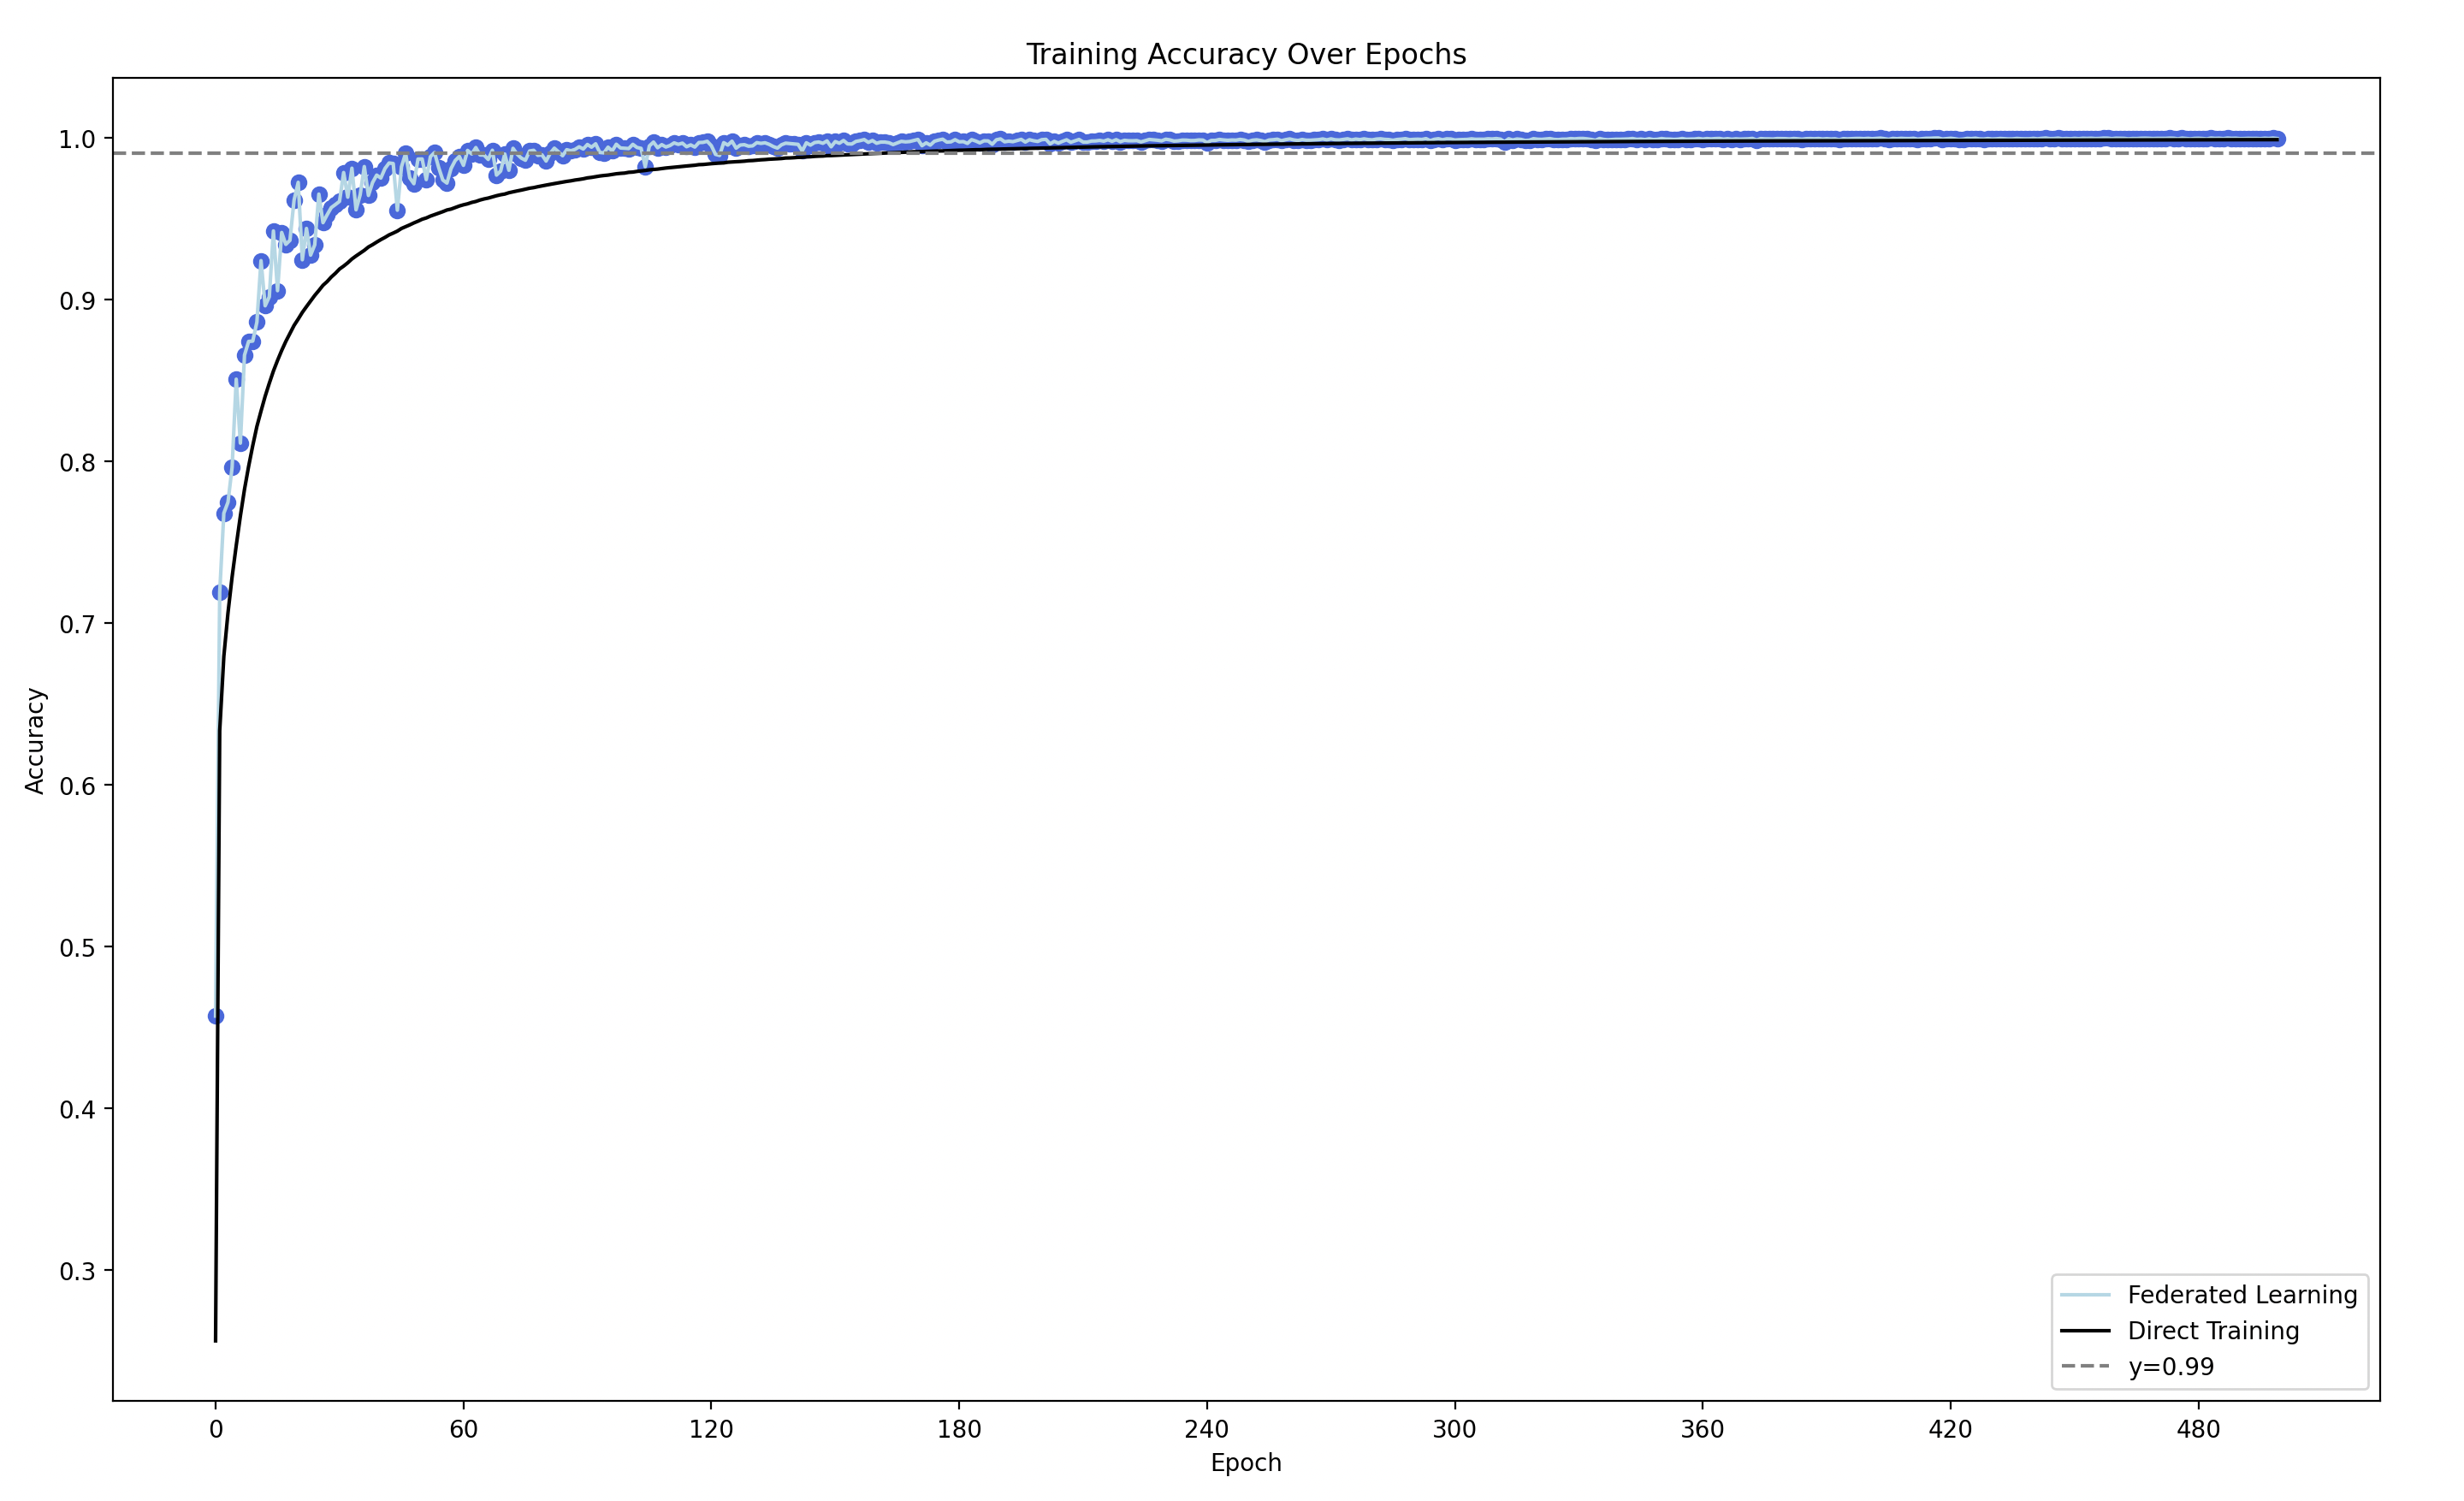
\includegraphics[width=1\textwidth]{1.png} % 插入图片
	      \vspace{-0.8cm}
        \caption{500 epochs}
    \end{minipage}
    \hfill
	%   \hspace{0.1\textwidth} % 调整这里的值来改变两张图片之间的间距
    \begin{minipage}[t]{0.49\textwidth}
        \centering
        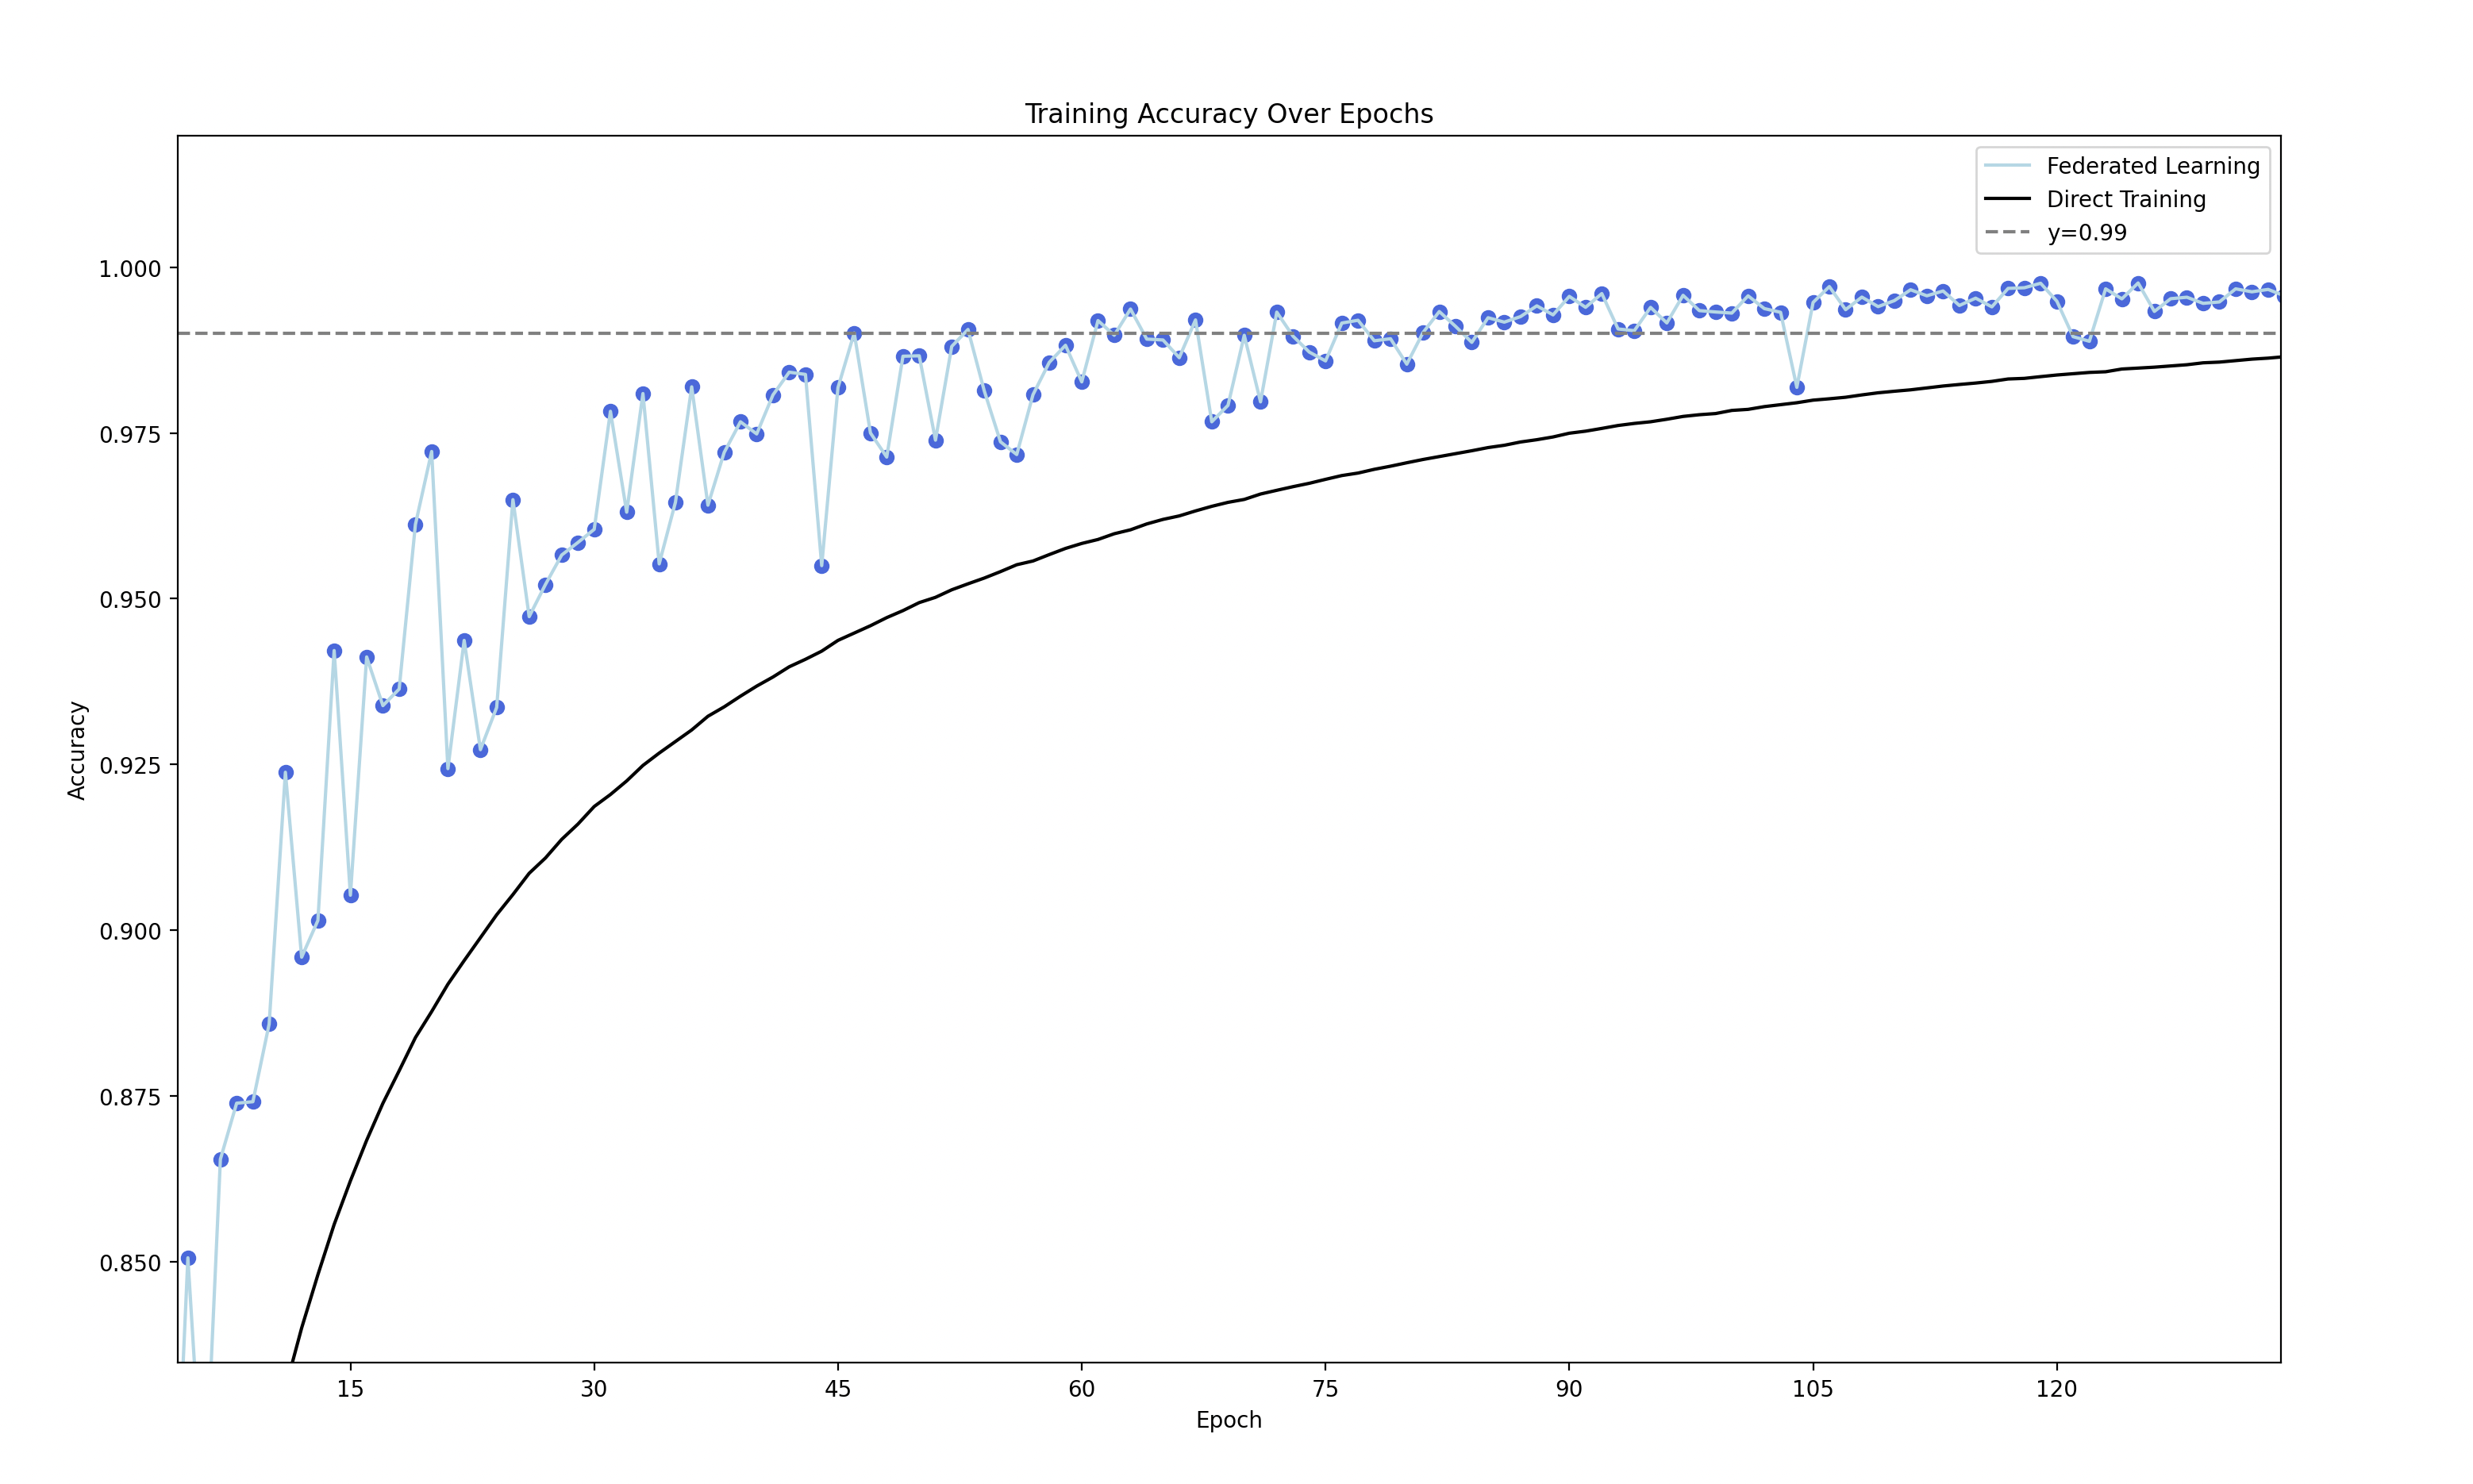
\includegraphics[width=1\textwidth]{2.png} % 插入图片
	      \vspace{-0.8cm}
        \caption{Enlarged figure}
\end{minipage}
\end{figure}
\\We can see that the data points are overwhelmingly above the line of y=0.99
 after 80 epochs. A more thorough analysis is listed below.
\subsection{Changing Epochs}
The following results are obtained by changing the number of epochs in the range of 
[1,5,10,20] and [1,5,10,20,50] while other hyperparameters remain the same, which are:
C = 0.1, num\_clients = 10, learning\_rate = 0.01, rounds = 50. The former has batch\_size 10 and 
the latter has batch\_size 50. The results are as follows:
\begin{figure}[htbp]
    \centering
    \begin{minipage}[t]{0.59\textwidth}
        \centering
        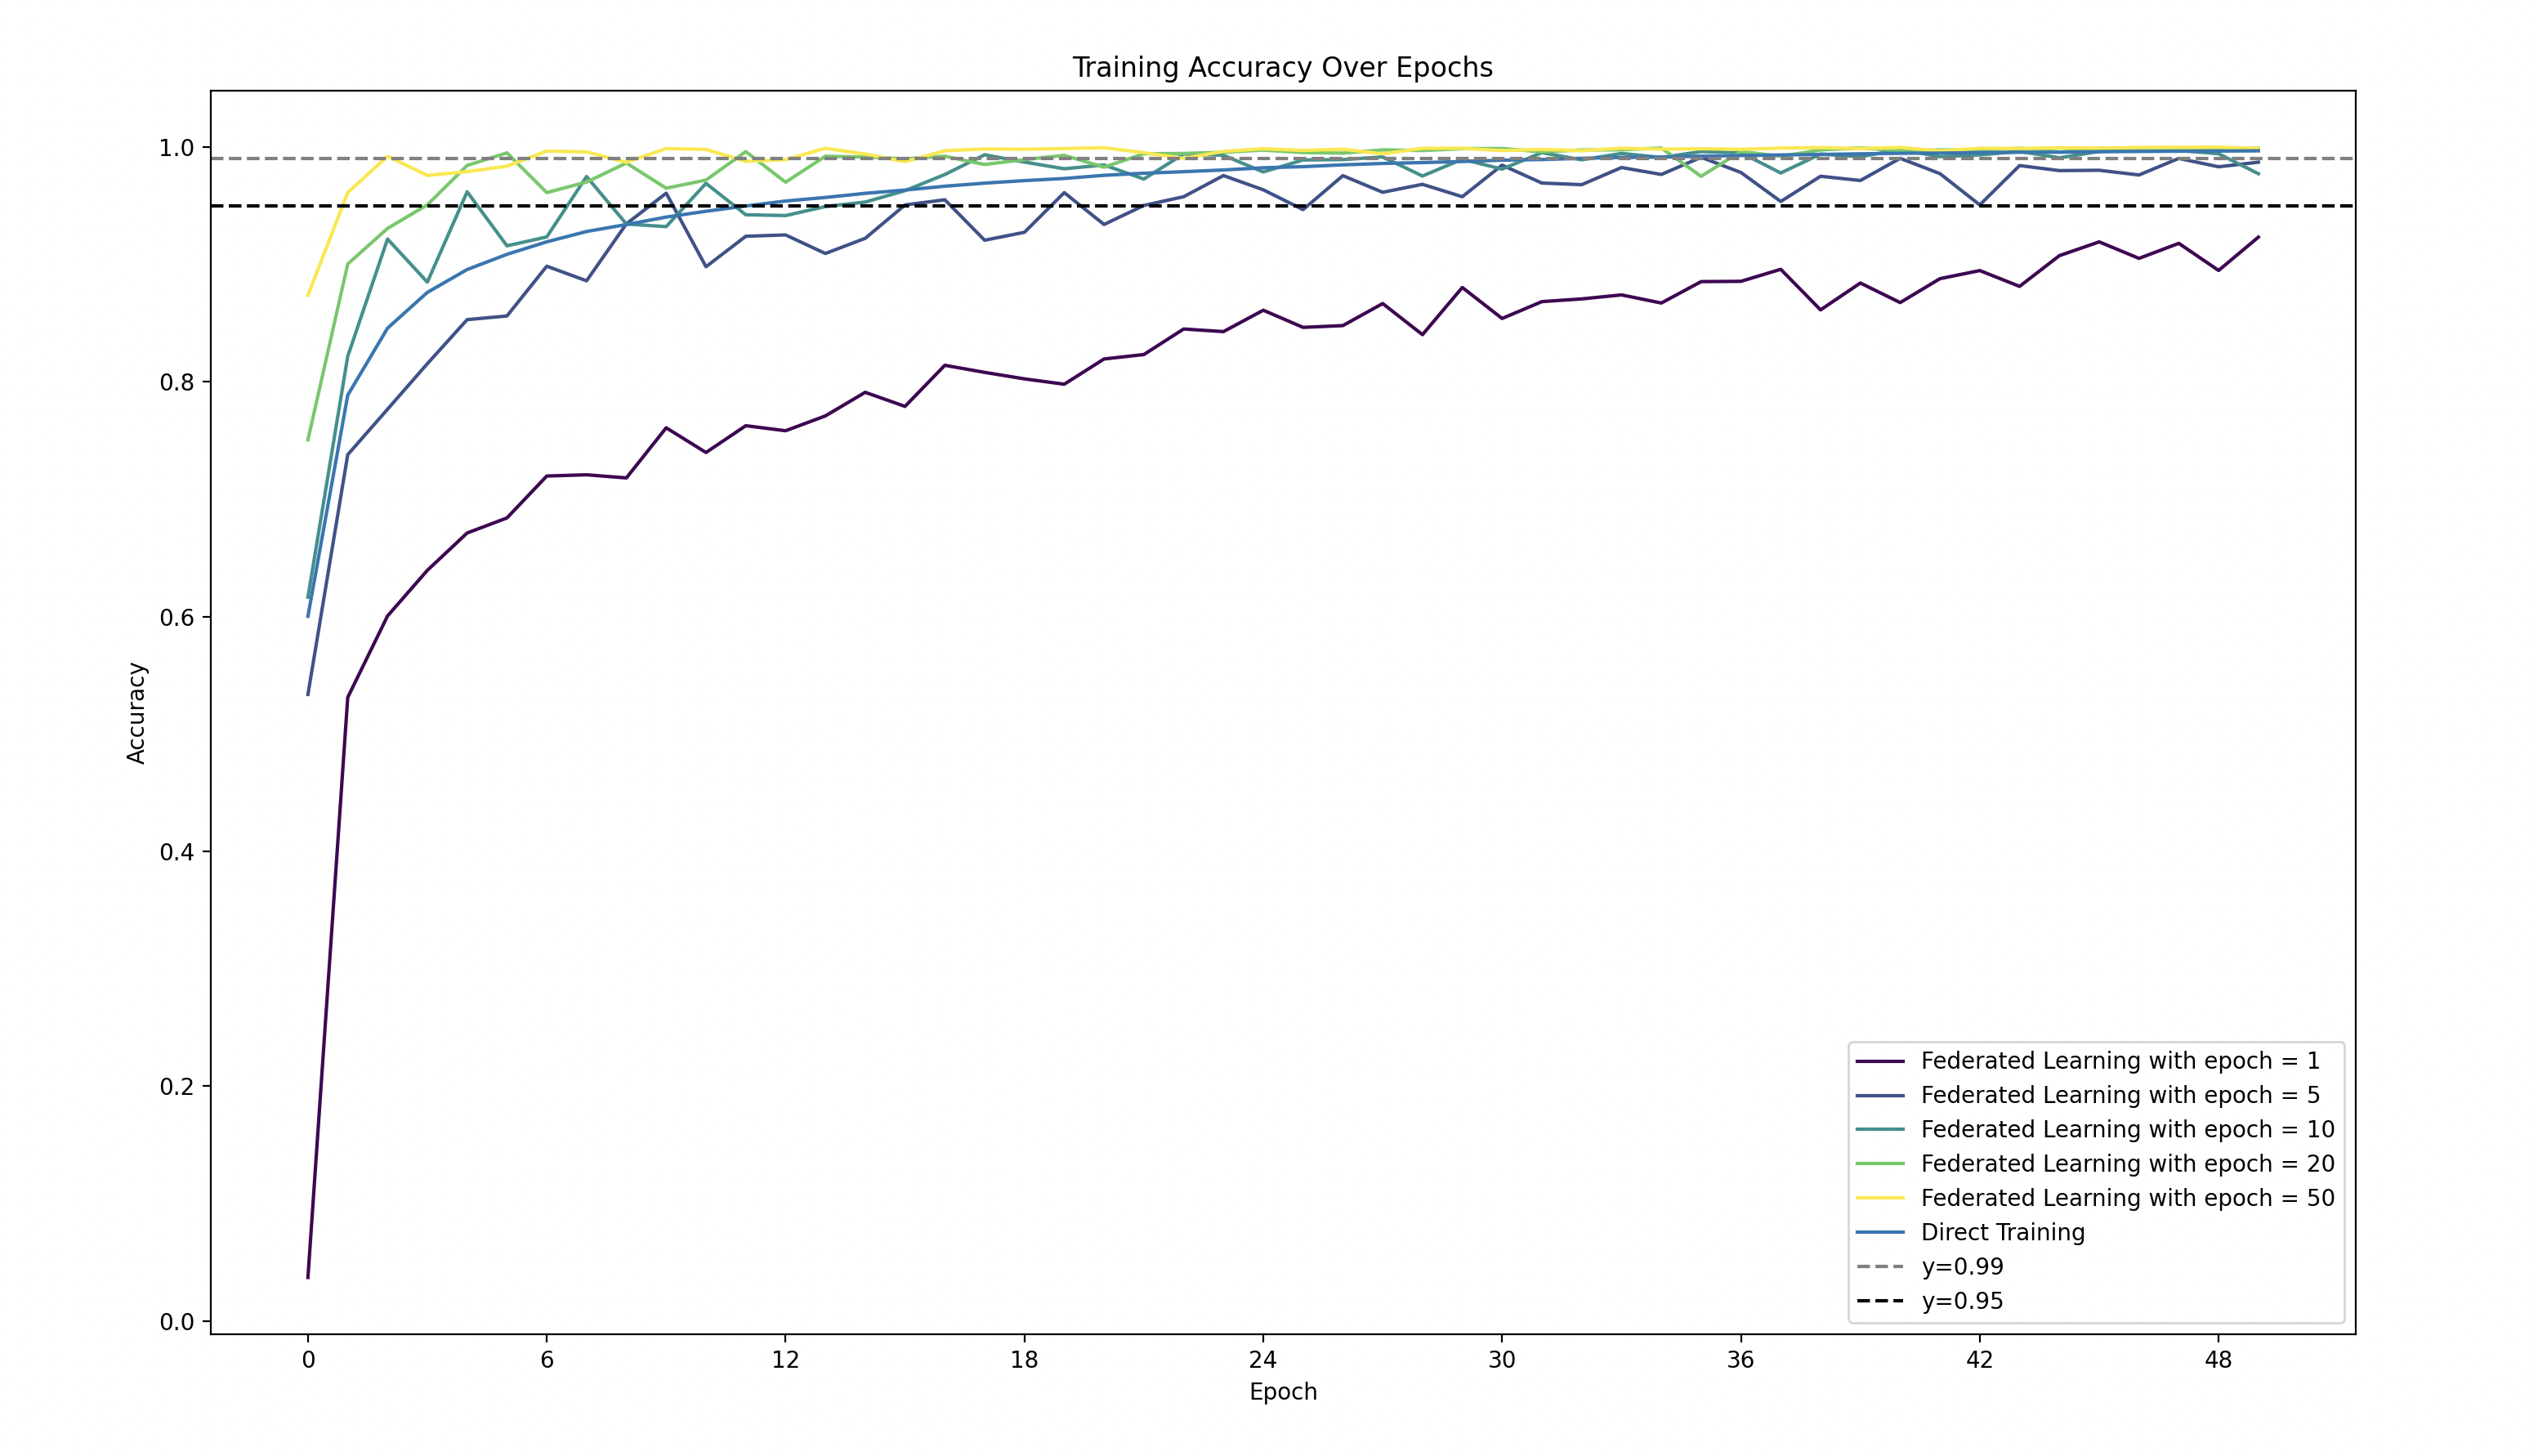
\includegraphics[width=1\textwidth]{batch10_epoch_change.png} % 插入图片
	      \vspace{-0.8cm}
        \caption{batch\_size=10}
    \end{minipage}
    \hfill
	%   \hspace{0.1\textwidth} % 调整这里的值来改变两张图片之间的间距
    \begin{minipage}[t]{0.4\textwidth}
        \centering
        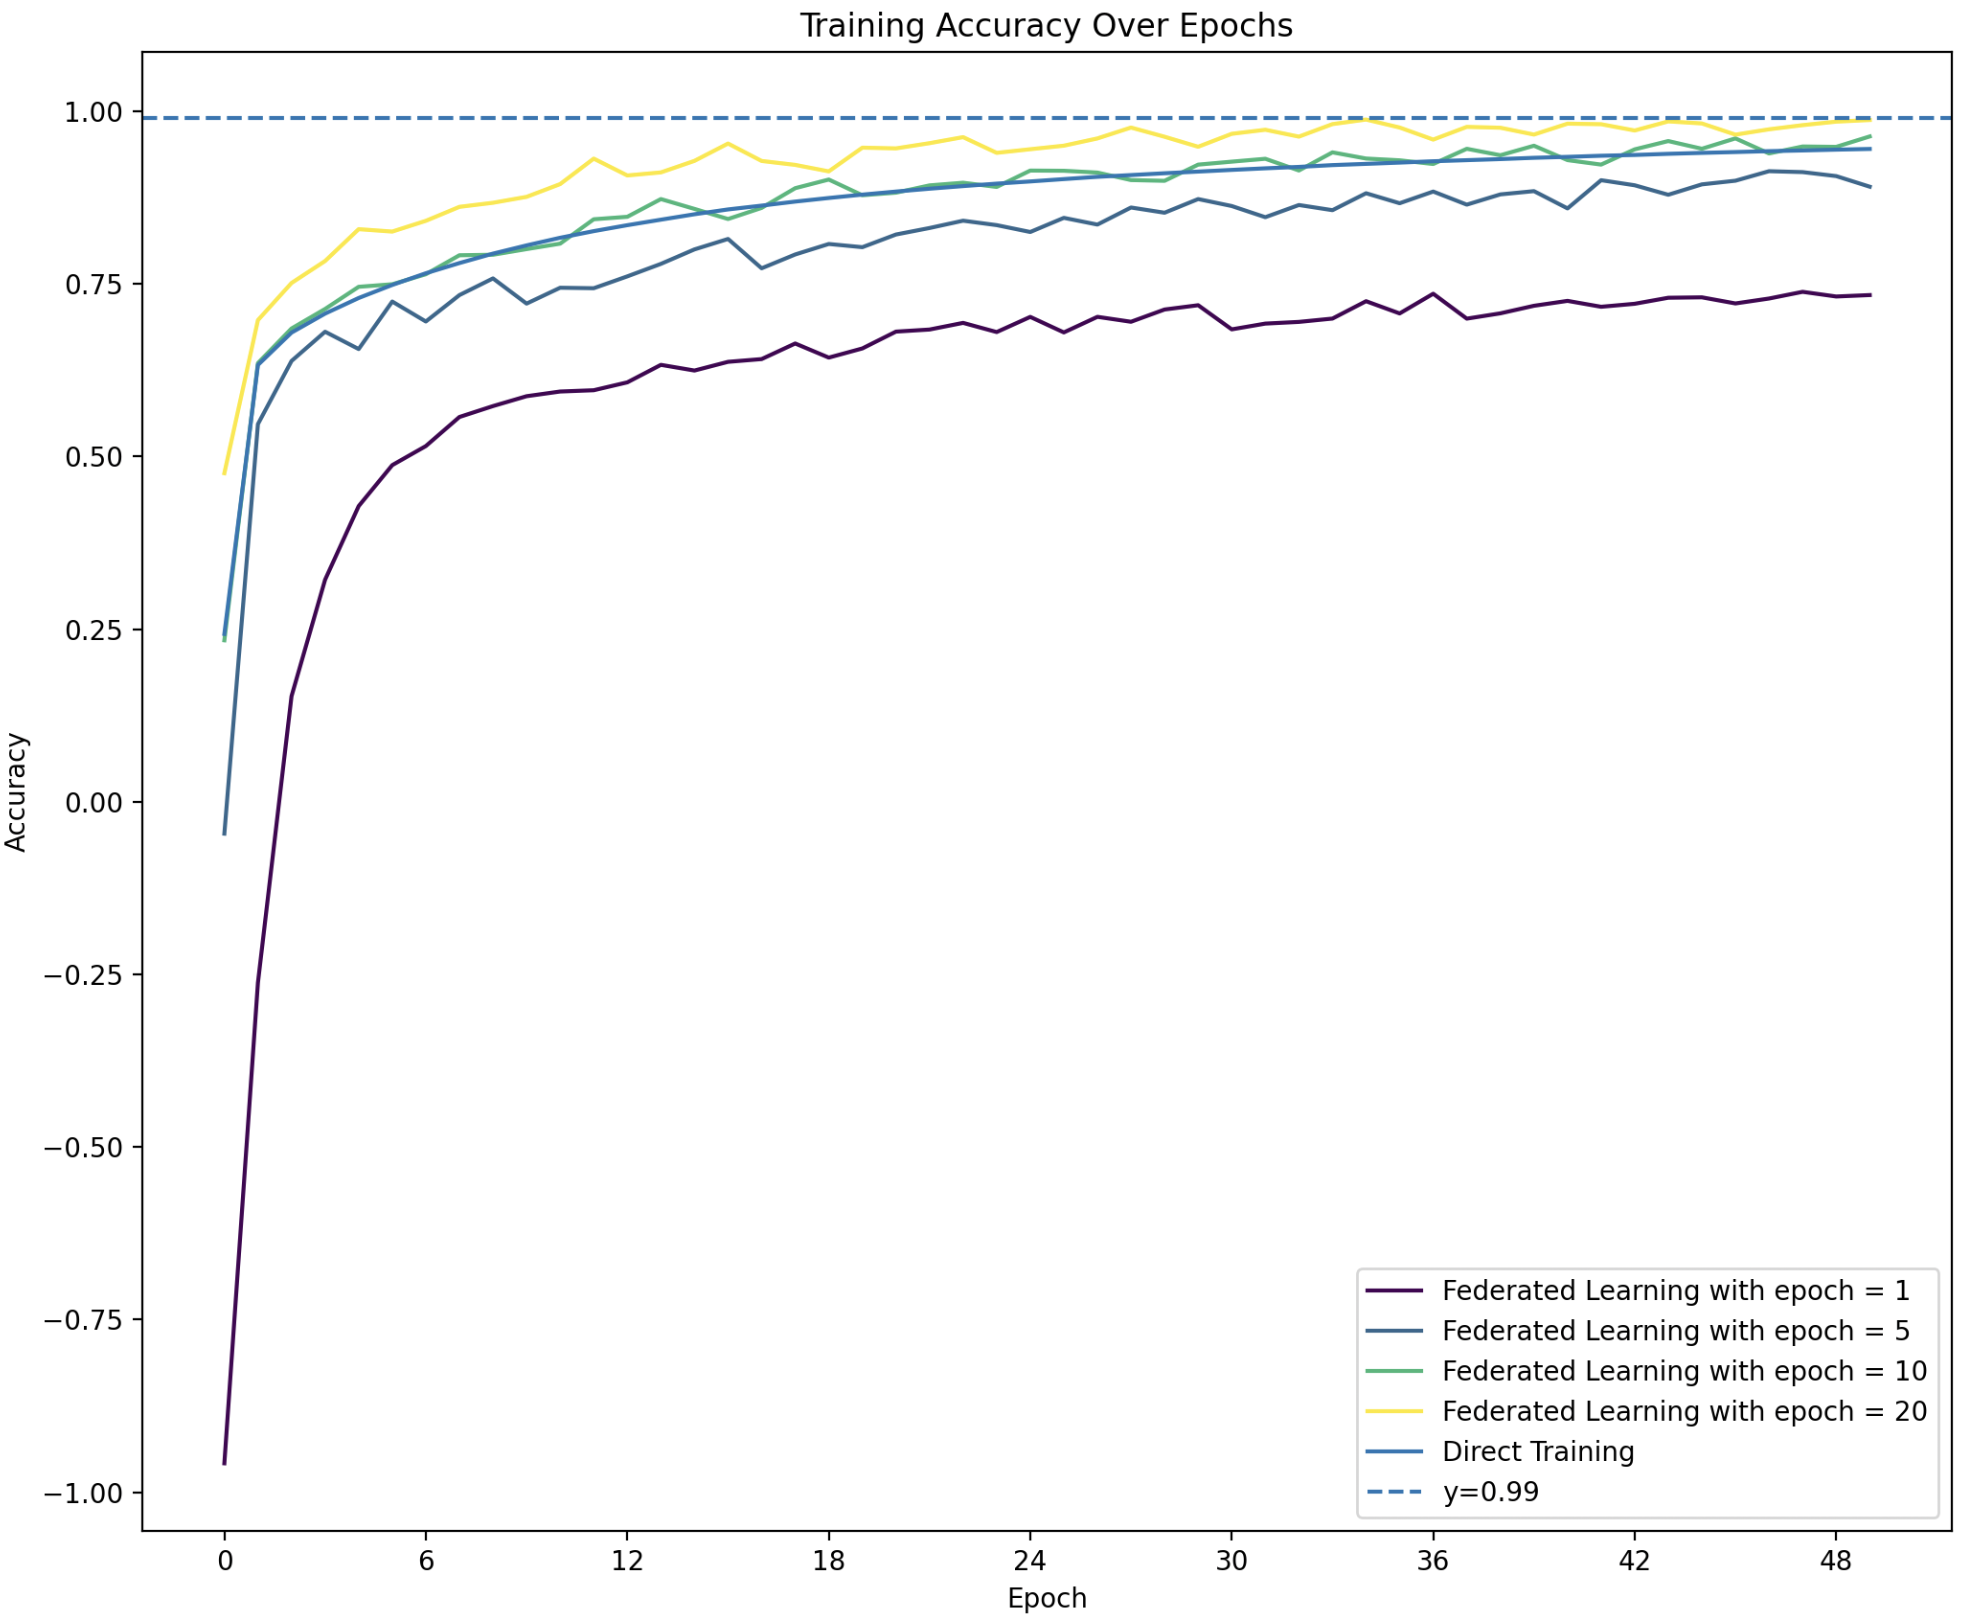
\includegraphics[width=1\textwidth]{batch64_epoch_change.png} % 插入图片
	      \vspace{-0.8cm}
        \caption{batch\_size=50}
\end{minipage}


\end{figure}
\\It is clear that Figure 3 shows a faster convergence than Figure 4, and 
among all the lines in Figure 3, convergence is the fastest when epoch=50.
Not only are the results consistent with the intuition that the more epochs the model is trained, the better the performance,
but also the results in the original paper, showing that the model reaches 99\% accuracy
after 34, 20, 18 rounds respectively for epochs 1, 5, 20.


\subsection{Changing \textit{C}}
The following results are obtained by changing the fraction of clients that are selected to participate in each round in the range of 
[0.0,0.1,0.2,0.5,1.0] while other hyperparameters remain the same, which are:
C = 0.1, num\_clients = 10, learning\_rate = 0.01, batch\_size = 64, rounds = 50. 
The results are shown in figure 5.\\
From the figure, all choices of C converge to 95\% accuracy after 25 rounds,
but oscillate around 99\% even around 50 rounds. It is hard to tell which choice of C
converge the fastest, but when computation time is taken into consideration, C = 0.1 seems to be the best choice.
\newpage
\begin{figure}[htbp]
    \centering
    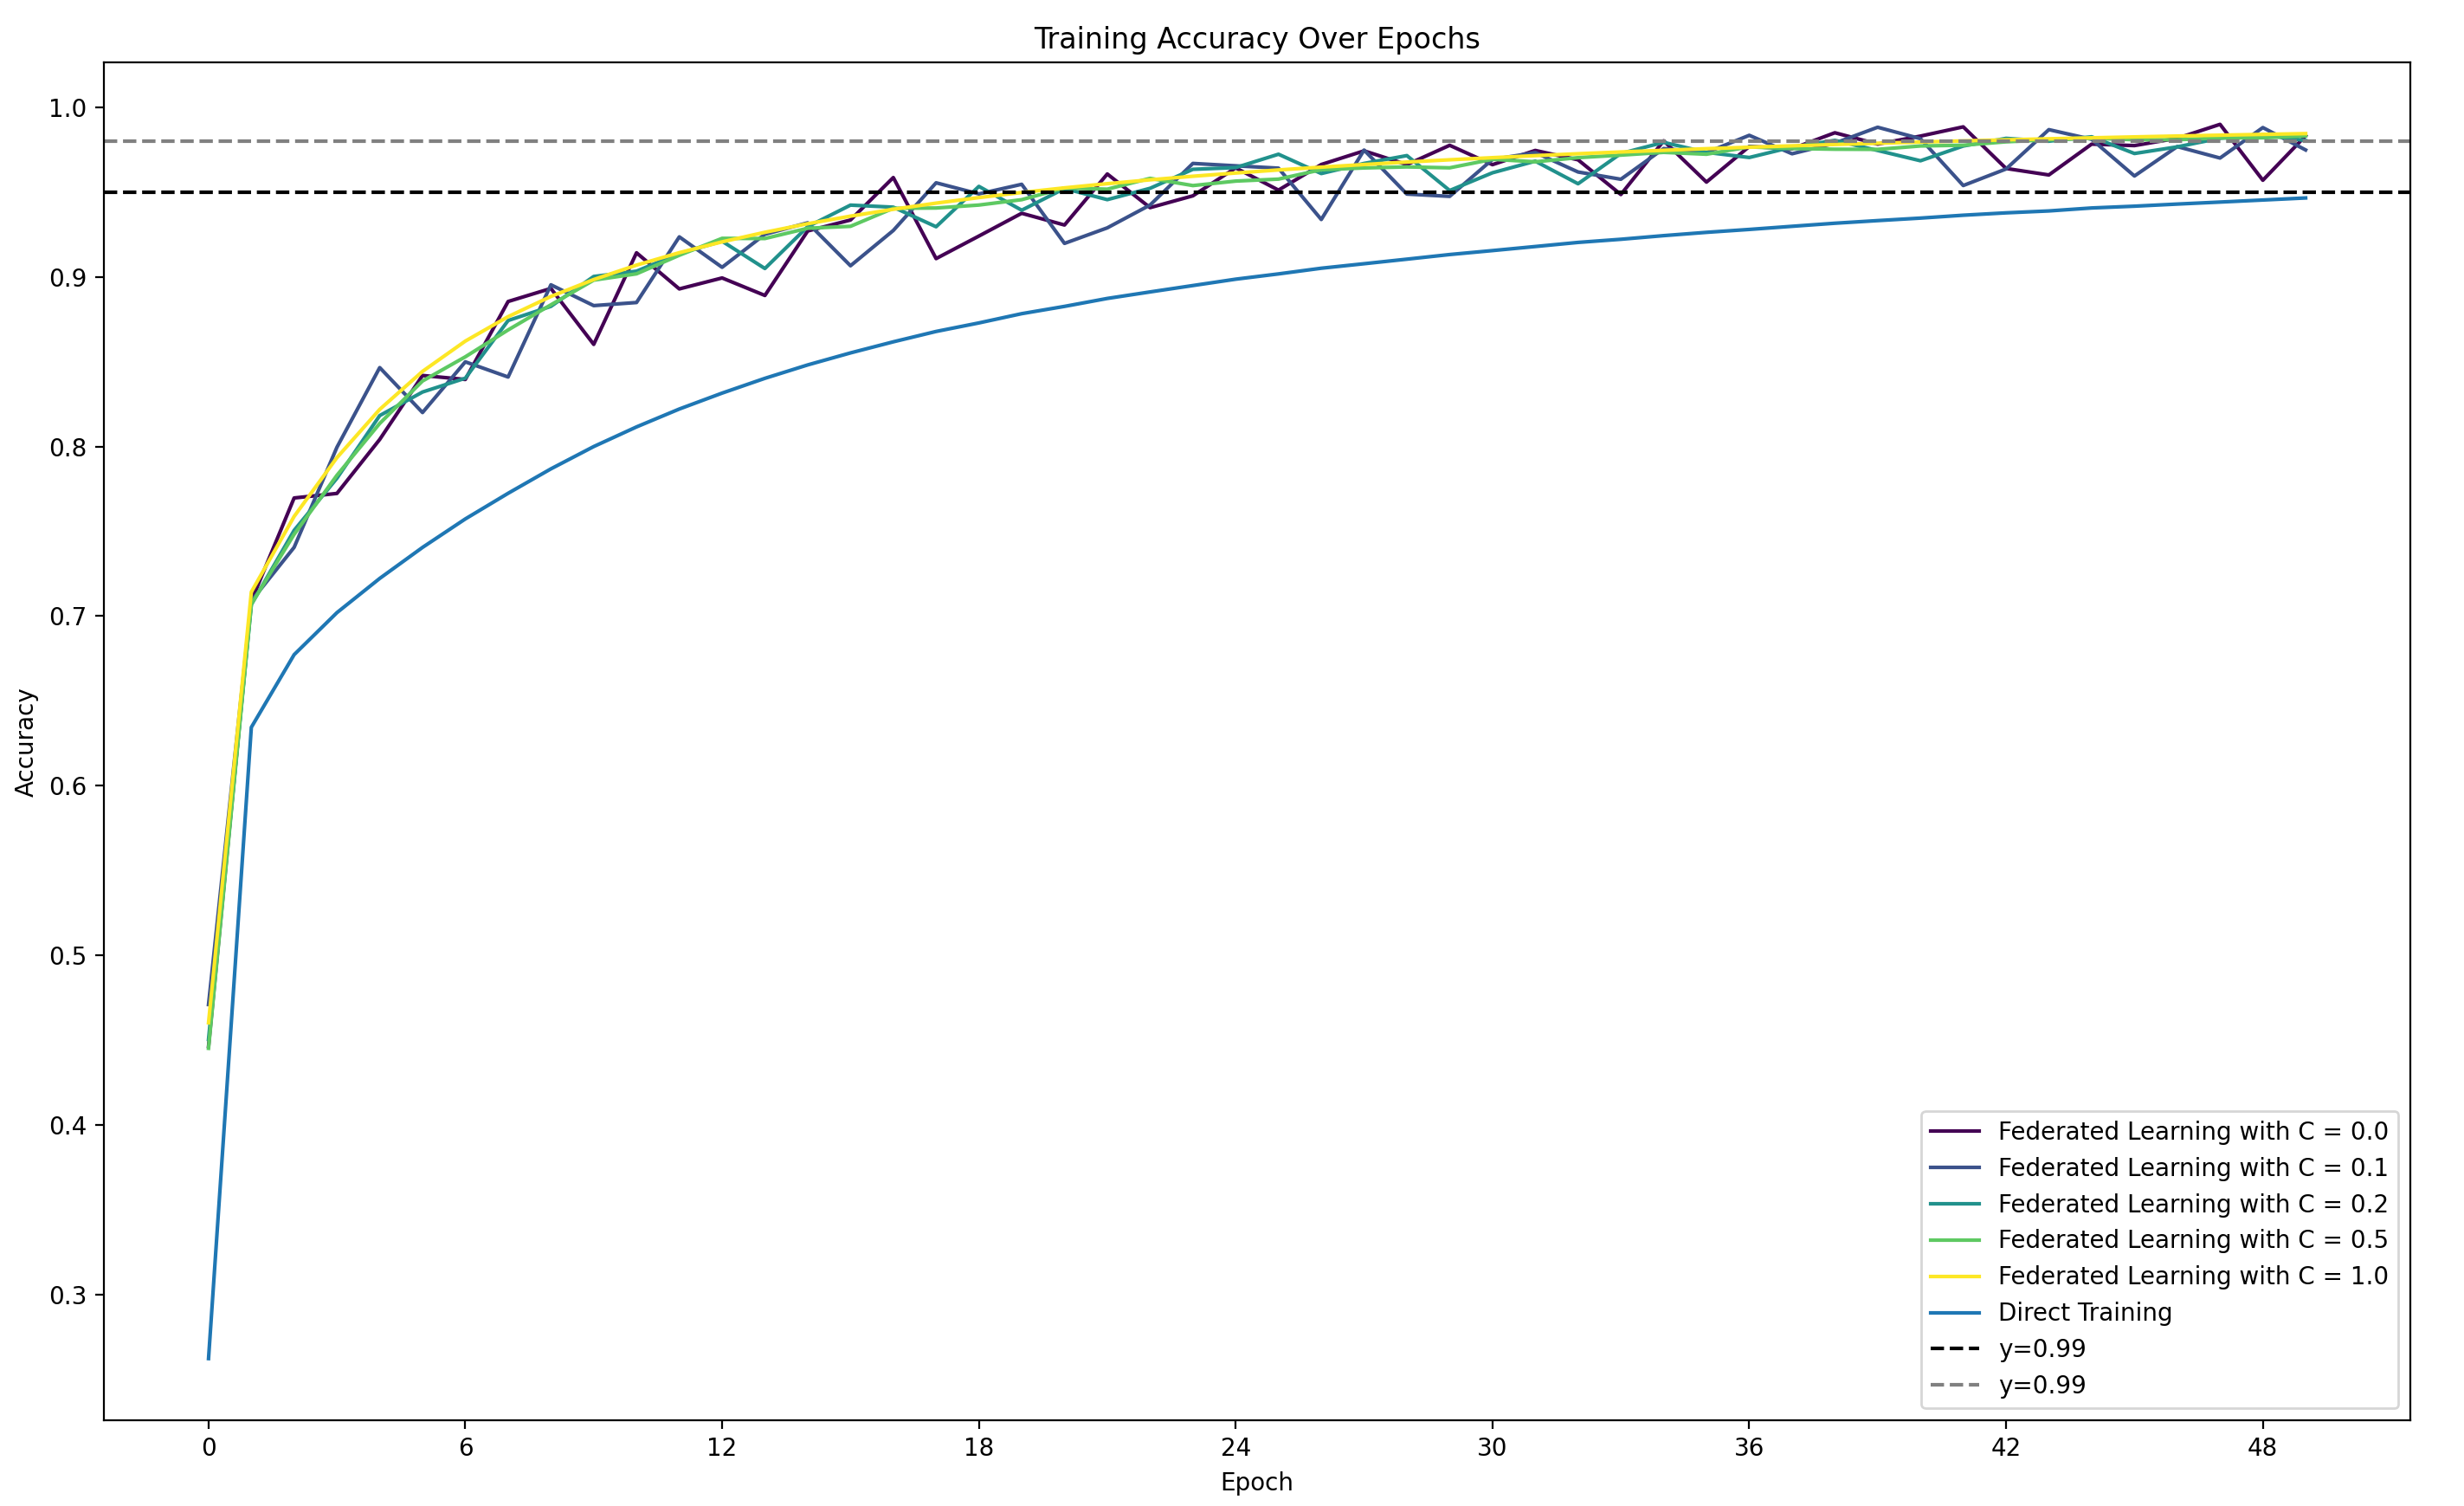
\includegraphics[width=1\textwidth]{C_change.png} % 插入图片
    \vspace{-1cm}
    \caption{Changes in C}
\end{figure}
\section{Reflections and Future Work}
In my replication, I have only trained the models using IID, whereas the quaintessence 
of Federated Learning lies in the heterogeneity of the data, namely the non-IID setting.
Also, it is surprising to see that the Federated Learning approach 
converges faster than the traditional centralized approach, the reason for which 
is still unclear to me.
\\
The mathematical approach with which to calculate the accuracy rate is also open to discussion.
In this article I robustly used $Accuracy = 1 - CrossEntropyLoss$ as the accuracy rate, which now seems to me 
naive and inaccurate. It maybe better to use the accuracy rate calculated from the test set. 
\\
Code optimization is also a problem. When compared to the direct SGD training, my 
Federated Learning approach converges much slower in reaching the desired accuracy rate.
\\
Finally, I haven't completely grasped how to utilize my gpu to accelerate the training process. In one 
training, it took RTX 4070ti 634 seconds to train 50 rounds, while i7-13700kf and Apple M2 respectively spent 519 and 419 seconds. 
% -----------参考文献 -------------------
\phantomsection
\addcontentsline{toc}{section}{参考文献} % 添加  "参考文献 " 到目录

%\setlength{\bibsep}{6pt plus 2pt}
\begin{thebibliography}{99}
    \bibitem{mcmahan2017communication} McMahan, H. Brendan, et al. "Communication-efficient learning of deep networks from decentralized data." \textit{arXiv preprint arXiv:1602.05629} (2017).
    \bibitem{} Sebastian Raschka, Vahid Mirjalili. \textit{Machine Learning with Pytorch and Scikit-Learn}. China Machine Press, 2023.
\end{thebibliography}






\appendix
\section{Complete Code Implementation} 
\begin{lstlisting}[language=Python, caption=Complete Code Implementation]
import torch
import torch.nn as nn
import torch.optim as optim
from torchvision import datasets, transforms
from torch.utils.data import DataLoader, random_split
import matplotlib.pyplot as plt
from matplotlib.ticker import MaxNLocator
import itertools
import copy
import random
import time

class SimpleNN(nn.Module):
    def __init__(self):
        super(SimpleNN,self).__init__()
        self.fc1 = nn.Linear(28*28,128)
        self.fc2 = nn.Linear(128,10)
    
    def forward(self,x):
        x = x.view(-1,28*28)
        x = torch.relu(self.fc1(x))
        x = self.fc2(x)
        return x
    
def get_data_loaders(batch_size,num_clients):
    transform = transforms.Compose([transforms.ToTensor(),transforms.Normalize((0.5,),(0.5,))])
    dataset = datasets.MNIST(root='./data',train=True,download=True,transform=transform)

    client_datasets = random_split(dataset, [len(dataset) // num_clients] * num_clients)
    client_loaders = [DataLoader(ds,batch_size=batch_size,shuffle=True) for ds in client_datasets]
    return client_loaders

def client_update(client_model,optimizer,train_loader,epochs):
    client_model.train()
    epoch_losses = []
    for epoch in range(epochs):
        total_loss = 0
        for data,target in train_loader:
            optimizer.zero_grad()
            output = client_model(data)
            loss = nn.CrossEntropyLoss()(output,target)
            loss.backward()
            optimizer.step()
            total_loss += loss.item()
        average_loss = total_loss/len(train_loader)
        epoch_losses.append(average_loss)
    return epoch_losses

def average_weights(global_model,client_models):
    global_dict = global_model.state_dict()
    for k in global_dict.keys():
        global_dict[k] = torch.stack([client_models[i].state_dict()[k].float() for i in range(len(client_models))],0).mean(0)
    global_model.load_state_dict(global_dict)  # Update the global model

def plot_losses(federated_losses, direct_losses):
    num_rounds = len(federated_losses)
    num_clients = len(federated_losses[0])
    
    # Plot the curve using Federated Learning
    avg_losses = []
    avg_accuracies = []
    for round in range(num_rounds):
        round_losses = federated_losses[round]
        flat_round_losses = list(itertools.chain(*round_losses))
        avg_loss = sum(flat_round_losses) / len(flat_round_losses)
        avg_accuracy = 1 - avg_loss
        avg_accuracies.append(avg_accuracy)
        avg_losses.append(avg_loss)
        plt.scatter(round,1-avg_loss, color='royalblue', marker='o')


    plt.plot(range(num_rounds), avg_accuracies, color='lightblue', linestyle='-', label='Federated Learning')


    for i in range(len(direct_losses)):
        direct_losses[i] = 1 - direct_losses[i]
    # Plot the curve using traditional SGD
    plt.plot(direct_losses, label='Direct Training', linestyle='-', color='black')
    
    plt.xlabel('Epoch')
    plt.ylabel('Accuracy')
    plt.title('Training Accuracy Over Epochs')
    # plt.ylabel('Loss')
    # plt.title('Training Loss Over Epochs')

    plt.axhline(y=0.99, color='grey', linestyle='--', label='y=0.99')

    plt.legend()
    plt.gca().xaxis.set_major_locator(MaxNLocator(integer=True))
    plt.show()

def direct_training(epochs=20):
    batch_size = 64
    learning_rate = 0.01

    model = SimpleNN()
    train_loader = get_data_loaders(batch_size, 1)[0]
    optimizer = optim.SGD(model.parameters(), lr=learning_rate)
    criterion = nn.CrossEntropyLoss()
    losses = []

    for epoch in range(epochs):
        total_loss = 0
        for data, target in train_loader:
            optimizer.zero_grad()
            output = model(data)
            loss = criterion(output, target)
            loss.backward()
            optimizer.step()
            total_loss += loss.item()
        average_loss = total_loss / len(train_loader)
        losses.append(average_loss)
        print(f"SGD training epoch {epoch+1} comlete, average loss:{average_loss}")

    return losses

def federated_learning(rounds=20):

    num_clients = 10
    batch_size = 64
    learning_rate = 0.01
    epoch = 20
    C = 0.1

    global_model = SimpleNN()
    client_loaders = get_data_loaders(batch_size, num_clients)
    all_client_losses = []

    for round in range(rounds):
        client_models = [SimpleNN() for _ in range(num_clients)]
        for client_model in client_models:
            client_model.load_state_dict(global_model.state_dict())
        
        optimizer = [optim.SGD(model.parameters(), lr=learning_rate) for model in client_models]
        round_losses = []

        # Randomly select clients to participate in the round
        m = max(int(C * num_clients), 1)  # Choosing at least 1 client
        selected_clients = random.sample(range(num_clients), m)

        client_losses = []
        for i in selected_clients:
            client_losses = client_update(client_models[i], optimizer[i], client_loaders[i], epoch)
            round_losses.append(client_losses)
        
        average_weights(global_model, [client_models[i] for i in selected_clients])
        print(f"Federated Learning round {round+1} complete, average loss:   {sum(client_losses)/len(client_losses)}")
        all_client_losses.append(round_losses)
    
    return all_client_losses

def main():
    rounds = 500

    start_time = time.time()
    federated_losses = federated_learning(rounds)
    direct_losses = direct_training(rounds)
    print("Time elapsed: ", time.time() - start_time)
    plot_losses(federated_losses, direct_losses)

if __name__ == "__main__":
    main()
  \end{lstlisting}
% \begin{enumerate}%[label={\rm (\arabic*)}]%\roman
% 	\item 第一项
% 		\begin{enumerate}
% 			\item 
% 			\item 
% 		\end{enumerate}
% 	\item 
% \end{enumerate}


% 这是一个不计数的列表.
% \begin{itemize}%[label={$\bullet$}]
% 	\item 
% 	\begin{itemize}
% 		\item 
% 		\item 
% 	\end{itemize}
% 	\item 
% \end{itemize}








\end{document} 